\chapter{The design process}
\label{ch:design}

\section{Requirements}

The Children and Youth Clinic expects an application where the user can view personally targeted procedures. These will feature the user's own personal avatar along with information about an upcoming procedure at the hospital. Afterwards, the user should be able to rate their experience, and if possible, this rating should be reflected when the procedure is shown in retrospect.

The target group will be children and youth at the clinic with ages raging from 5 to 12. The content of the application must therefore be adapted to the target group and be suitable for their age. An essential plan when it comes to the design of the application is to let children of the intended age group test it in various stages of its development. Their input is valuable since it can contribute to making the application age-appropriate \parencite{stalberg2016}.

The clinic expressed that they intend to use the application on larger screens and most likely on tablets.

\section{The first design}

The PictogramApp application, of which the master project will primarily be based on, allows users to create their own \emph{stories} consisting of an arbitrary number of \emph{scenes}. These concepts can be applied to the new application, though they will be named as \emph{procedures} and \emph{steps} respectively. Contrary to the original application, a single step may be animated and contain more information than a single picture can provide.

Some initial sketches were made during the first meeting with Paul Thorsen. Among others, they illustrated a list of procedures, a procedure in its entirety, rating the procedure and how the rating is reflected in the list of procedures. Selected sketches were used as a basis for the initial designing process.

\begin{figure}
    \centering
    \begin{subfigure}{0.95\textwidth}
        \centering
        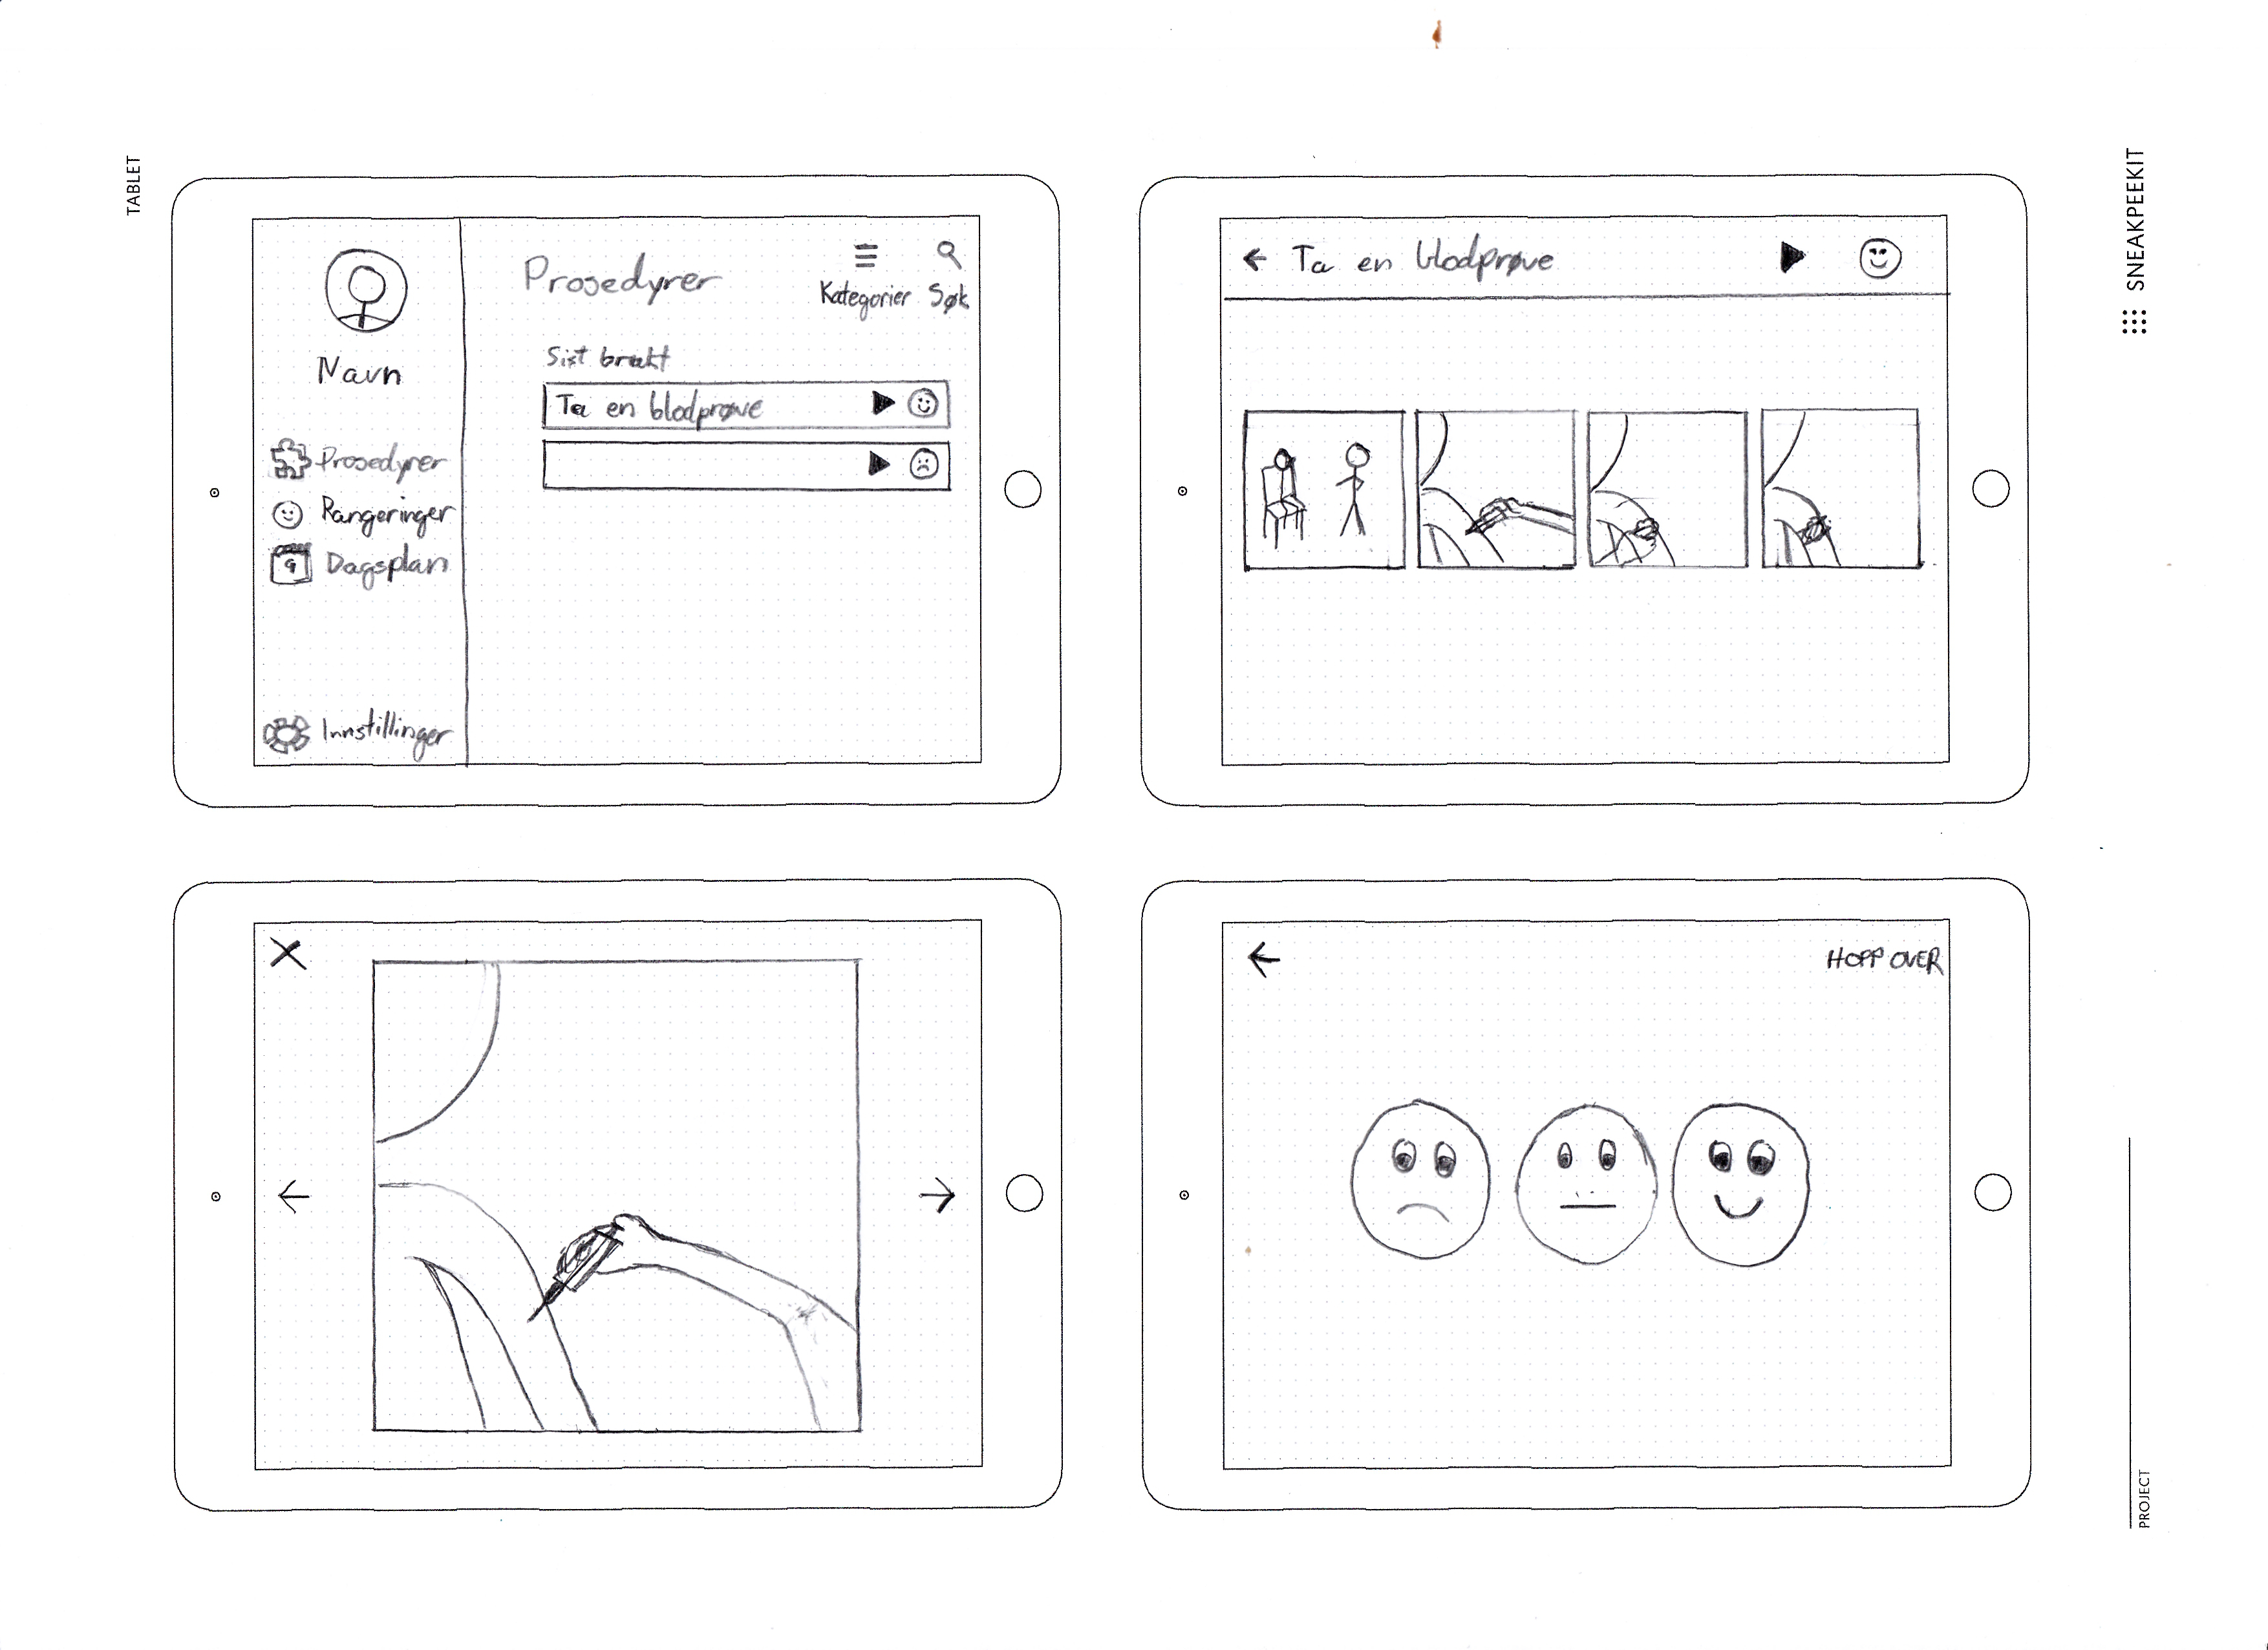
\includegraphics[width=\textwidth]{20181114_0001.jpg}
        \subcaption{Viewing a procedure}
        \label{fig:sketch-viewprocedure}
    \end{subfigure}
    \begin{subfigure}{0.95\textwidth}
        \centering
        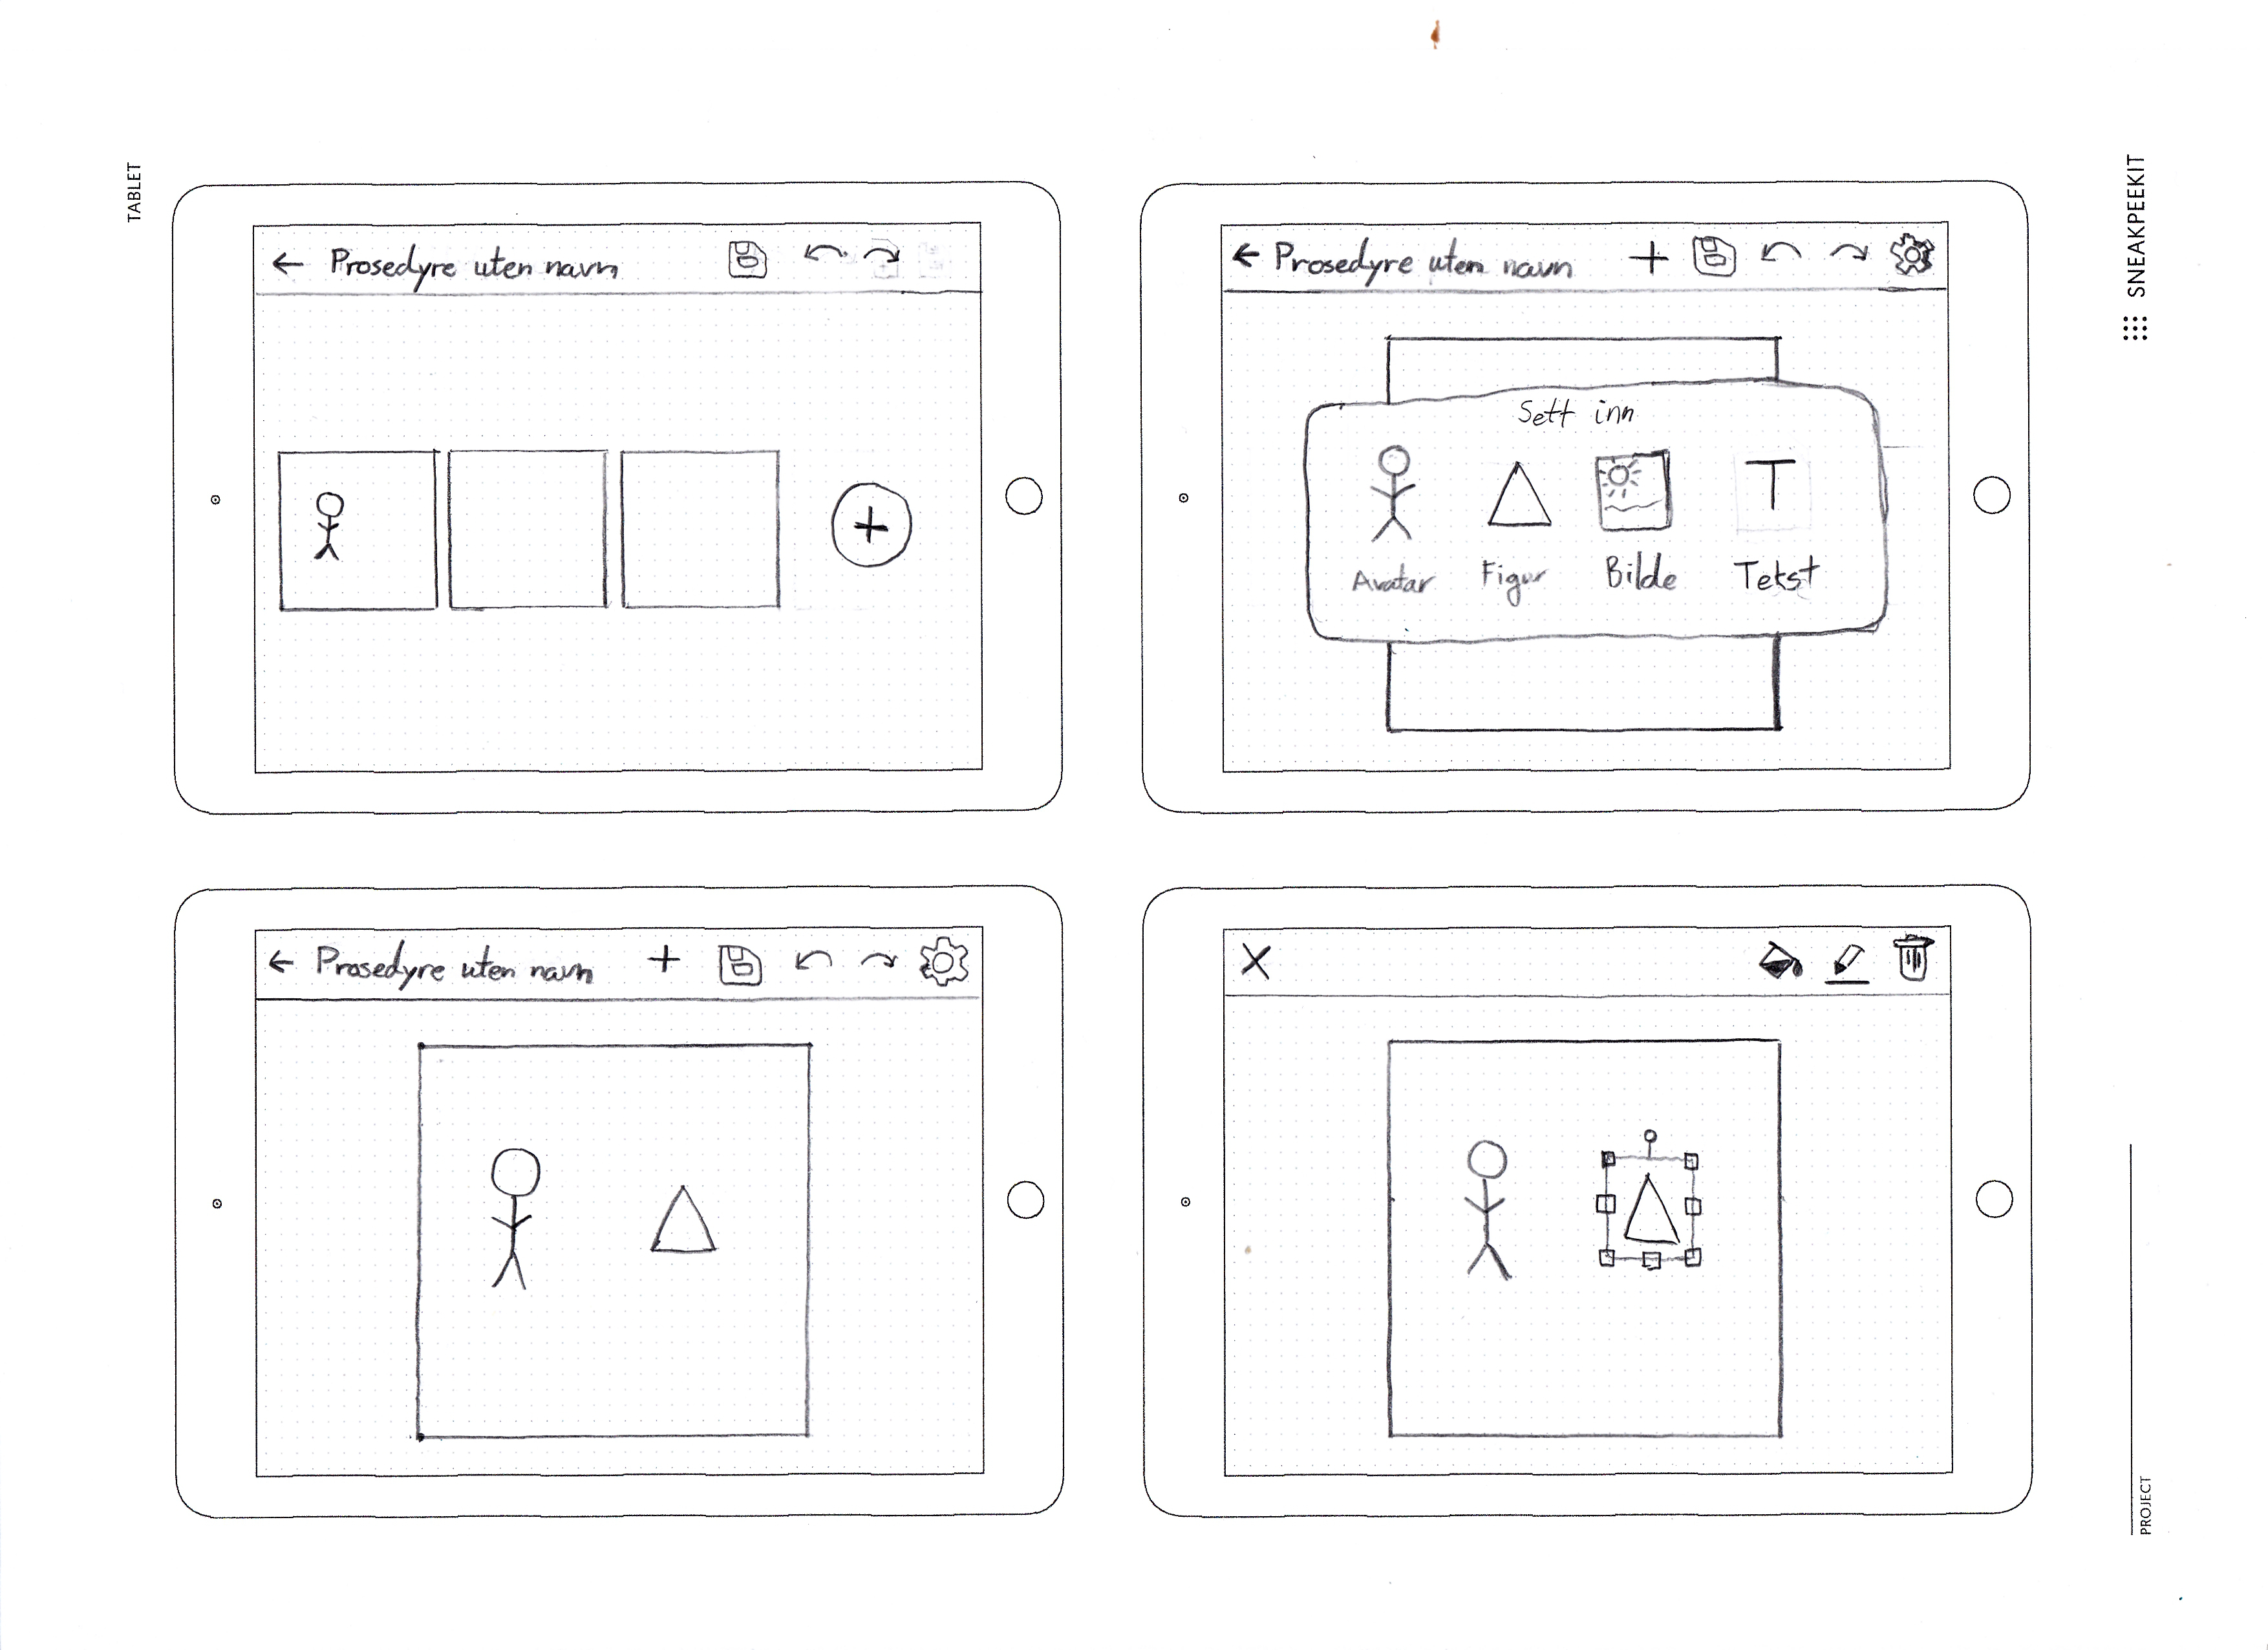
\includegraphics[width=\textwidth]{20181114_0002.jpg}
        \subcaption{Editing a procedure}
        \label{fig:sketch-editprocedure}
    \end{subfigure}
    \caption{Sketches of the first design}
    \label{fig:sketch-firstdesign}
\end{figure}

The first design shows the user entering a procedure and evaluating it (see figure \ref{fig:sketch-viewprocedure}), a common use case in this application. When viewing a procedure, its steps are shown in an horizontal, scrollable sequence of pictures. The user will be able to scroll across the whole procedure from left to right and to put each picture in focus, essentially becoming a step-to-step tutorial. This is a good way to get an overview of the procedure on its own, but it provides less interaction than if the user would, say, walk through the steps in a game-like approach. At the end of the procedure, the user is prompted to express their experience through use of smileys, a method proven to be quite successful \parencite{stalberg2016}. A more complicated system for rating procedures and experiences has been suggested but such a system is not within the scope of this application.

There are also several sketches showing how the procedure may be edited by an administrator (figure \ref{fig:sketch-editprocedure}). Creating and modifying procedures on a tablet is one possibility, although not the only one, given the tablet requirement. Compared to PictogramApp, the interface is supposed to be more drag-and-drop oriented with possibilities to drag pages between each other. Another change is that elements must be clicked/tapped before they can be modified.

\subsection{Considerations}

The scope of the application had been partially accounted for at this stage. It was clear that the application would be used to inform patients about upcoming procedures and let patients rate them afterwards. However, it was not known whether it was intended to be used during procedures and in context with a health professional.

Children at this age have most likely been made known to tablets and interactive devices, but the youngest children of the target group may not have sufficient prior experience, either due to their age or health-related issues or a combination of both. Less experienced users should be able to learn how to use the application quickly regardless. It is therefore a good idea to consider ways to inform and possibly demonstrate the user about possible ways to interact with the application.

These initial ideas to the design will only give an indication of the final visual style of the application. Depending on the feedback of the test groups, the style should be one that the users feel more interesting. Some possible visual styles include a modern and minimal approach with focus on essential elements (similar to PictogramApp) and a more cartoonish, fun style with drawing-like pictures and an informal look. Regardless of what style is chosen, it should fit to the style of the avatars that are already made.



\section{Prototyping the design}

Although the design had been iterated over several times, only the third and fourth designs had hotspots which allow the user to navigate across the different screens. These were used in discussions with the supervisor, Paul Thorsen and Avans.




Concerns
